\documentclass[debug]{rmaa}

%%%
%%% Load any optional packages you need here with \usepackage
%%% 
\usepackage{amsmath}

% This allows compact, in-paragraph, and as-paragraph  versions of the
% standard itemize and enumerate environments. 
\usepackage{paralist}

% These are used in one of the graphics examples
\usepackage{psfrag,color}

% Allow accented characters to be entered directly
\usepackage[latin1]{inputenc}

%%%
%%% Define any personal macros here
%%% 

% These are some I use in typesetting example code
\newcommand{\bs}{\textbackslash}
\newcommand{\CS}[1]{\texttt{\textbackslash #1}}
\newenvironment{Example}
{\begin{list}{}{\setlength{\leftmargin}{10pt}\setlength{\rightmargin}{10pt}}%
  \item[]\itshape}
  {\end{list}}

  
%%%
%%% Article preamble commands (title, authors, abstract, etc.) 
%%% None of these produce any output themselves, they just set things 
%%% up for \maketitle
%%%

% Please use mixed case here, since this title gets propagated onto
% the web page, ADS entry, etc. 
\title{Velocity dispersion of NGC-6366} 

% For the conference proceedings, the author affiliations should be
% subscripted, using \altaffil and/or \altaffilmark + \altaffiltext
% Note that \altaffilmark goes after a comma and that `and' is spelt
% out.
\author{
  V. Lora \altaffilmark{1} and
  F. J. S\'anchez-Salcedo,\altaffilmark{2}}

% Note that \altaffil, \altaffilmark go inside the scope of the
% \author{...} command but \altaffiltext is outside it. 
\altaffiltext{1}{Instituto de Radioastronom\'\i{}a y Astrof\'\i{}sica,
  UNAM, M\'exico.}

\altaffiltext{2}{Instituto de Astronom\'\i{}a,
  UNAM, M\'exico.}


% Authors for running headers - surnames only, et al. if more than 3. 
\shortauthor{Lora \& S\'anchez-Salcedo}
% Title for running header
\shorttitle{velocity dispersion of NGC-6366}

% Full postal addresses (in alphabetical surname order!)
% plus email addresses in parentheses. 
\fulladdresses{
\item V. Lora: Instituto de Radioastronom\'\i{}a y
  Astrof\'\i{}sica, Universidad Nacional Aut\'onoma de M\'exico,
  Apartado Postal 3--72, 58090 Morelia, Michoac\'an, M\'exico
  (v.lora@irya.unam.mx).
  
  \item F. J. S\'anchez-Salcedo: Instituto de Astronom\'\i{}a, 
  Universidad Nacional Aut\'onoma de M\'exico,
  Apartado Postal 70--543, 04510 D. F., M\'exico
  (jsanchez@astro.unam.mx).}

% List of authors used to construct table of contents
\listofauthors{V. Lora\& F. J. S\'anchez-Salcedo}
% Each author in Surname, Initials format, used in generating Author
% Index entries.
\indexauthor{Lora, V.}
\indexauthor{S\'anchez-Salcedo, F. J.}

% English abstract
\abstract{Here the abstract}

% Spanish abstract - leave blank and it will be translated by the
% editors. 
\resumen{Aqui va el resumen}


% Keywords must be from the standard list and in alphabetical order. 
\addkeyword{Galaxy: Stellar clusters}
\addkeyword{Galaxy: Kinematics and Dynamics}
\addkeyword{Galaxy: Numerical simulations}


%%%
%%% Beginning of document proper
%%%
\begin{document}
% Typeset article header
\maketitle


\section{Introduction}
\label{sec:intro}

Articles to be considered for publication in the main journal should
be prepared in the ``manuscript'' style, which is now the
default when no explicit options are
given to the \CS{documentclass} command. The reason for this is to
allow authors to concentrate on the content of their paper, rather
than the details of the typesetting. This style also has ample margins
to allow a comfortable number of words per line and to leave room for
marginal notes.\\


In \S~\ref{sec:ngc-6366}, we present some properties of the GC
NGC-6366. In \S~\ref{sec:nbody} we describe the N-body code used 
for the simulations.  In \S~\ref{sec:results}, we give the results
from our N-body simulations. Finally, in \S~\ref{sec:conclusions}
we give our conclusions.


\newpage
\section{The globular cluster NGC-6366}
\label{sec:ngc-6366}

The GC NGC-6366 is one of the closest GCs to the Sun ($R_{_\odot}=3.6$~kpc), 
and it is located at a Galactocentric distance of $\sim5$~kpc \citep{chen:10}. 
In the new GAIA DR2 release \citep{helmi:18}, they report a position on the sky 
for NGC-6366 of $(\alpha , \delta)=(261.9393,-5.0752)�$.

This GC is classified as metal rich with $[Fe/H]=-0.55$ \citep{puls:18}, and it 
is very possible associated with the MW bulge (bulge GCs usually have 
$[Fe/H]>-1.3$; \citeauthor{bica:16} \citeyear{bica:16}). Another interesting feature 
of bulge GCs is, that they frequently pass through high density regions in the 
Galaxy, therefore they are subject of tidal stripping. The latter seems to be the 
case for NGC-6366. 

Its location in the inner parts of the Galaxy, makes it very likely 
to experience frequent gravitational interactions, which could lead to the depletion 
of low mass stars \citep{paust:09}. Furthermore, \citet{gnedin:97} compute a life 
time for NGC-6366 in the range of 1.15--6.3~Gyr, taking into account the evaporation 
of stars from the clusters, and the tidal shock from the Galactic bluge and disk.
In addition, \citet{chen:10} report that their (color magnitude diagram) CMD-selected 
members show clumpiness around NGC-6366, with the majority of the clumps distributed 
within its tidal radius ($15.20'$), which might be an indicator of tidal stripping.

\citet{campos:13} present multichromatic isochrone fits to the color-magnitude data 
of NGC-6366. They determined for this CG a foreground reddening $E(B-V)=0.69$, a 
distance modulus $(m-M)_{V}=15.02$, and an age of $11\pm1.15$~Gyr.
Interestingly, \citet{puls:18} suggest that NGC-6366 could contain a single stellar 
population, and in such a case it would give strenght to the idea that (at 
least in the Galaxy) single population GCs are brighter than $M_{V}\approx-7$.

( despite what \citealp{puls:18} mantains) 


\section{The velocity dispersion of NGC-6366}
\label{sec:vel_dispersion}

\cite{harris:96} (and an updated catalogue version \citealp{harris:10}) 
summerize the parameters for MW GCs, such as distances,
reddening, luminosity, dynamical parameters, etc. \cite{mclaughlin:05} extends
the latter cattalogue. They report structural and dynamical properties for $153$ 
spatially resolved star clusters in the MW, the Large Magellanic Cloud (LMC), 
the Small Magellanic Cloud (SMC), and the Fornax dwarf spheroidal (dSph) galaxy.

Particularly, this catalogue includes central velocity dispersions with which 
they derive dynamical mass-to-light ratios. Also, using publicly available 
population-synthesis models, they compute the V-band mass-to-light ratios for 
their complete $153$ cluster sample.  

In general the dynamical mass-to-light ratios and the mass-to-light ratios 
computed from population-synthesis compare well (see Fifure~XXX). However,
NGC-6466 is an outlier.




%Even in the Milky Way globular cluster
%system, reliable velocity-dispersion measurements and dynamical
%M/L ratios exist for fewer than half of the 85 clusters that we
%model here. 


%%%%%%%%%%%%%
%   Figura  %
%%%%%%%%%%%%%
\begin{figure}[!t]
\centering
  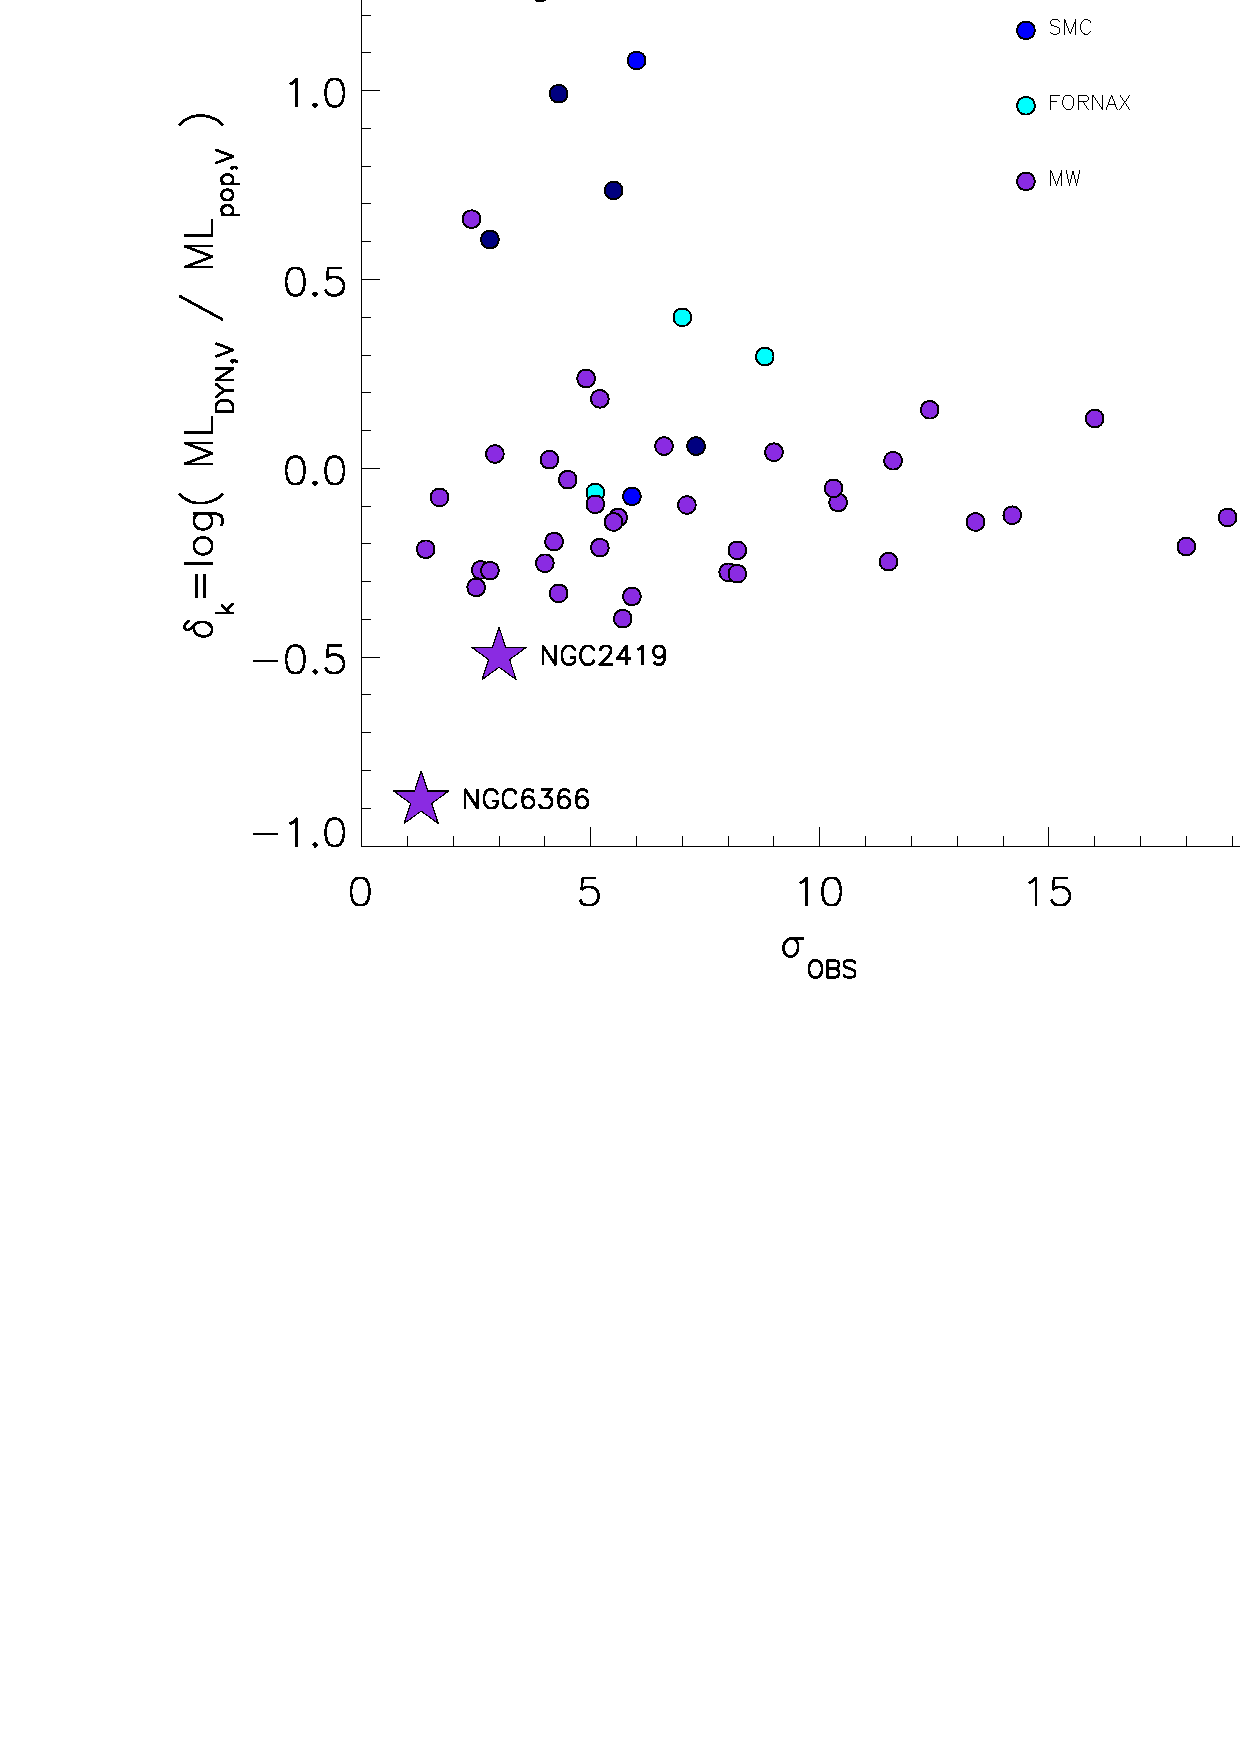
\includegraphics[width=0.6\columnwidth]{Delta}
  \caption{Example of a simple single-column figure.}
  \label{fig:simple}
\end{figure}


\section{The N-body code}
\label{sec:nbody}

We carried out $N$-body simulations of a star cluster and a central


\section{Results}
\label{sec:results}

For the initial mass density profile of NGC-6366 GC, we used a Plummer 
\citep{plummer11} mass density profile given by
\begin{eqnarray}
\rho_{c}(r) &=& \rho_{0} (1+r^2/r_p^2)^{-5/2} \mbox{ ,}
\label{eq:plummer}
\end{eqnarray}
where $r_p$ is the Plummer radius. We use the relation between the half-mass 
radius, and the plummer radius ($r_{h}=1.3 r_{p}$) to generate the initial
conditions of NGC-6366.


We first carried out an $N$-body simulation with the code described in 
section~\ref{nbody} using the initial condition given by equation \ref{eq:plummer}.

To the equations of motion in the $N$-body code, we then added the contribution
of the potential of a massive object $M_c$ located at the center of the stellar
cluster. We then carried out two simulations, model M1 with $M_c=0.1\,M_*$ and
model M2 $M_c=0.5\,M_*$ (where $M_*$ is the mass of the cluster). Since the
cluster is modeled with $10^3$ equal mass particles, these values of $M_c$
correspond to 100 and 500 times the mass of the individual particles.
We let the two models (M1 and M2) evolve from $t=0$ to $\sim 15$ crossing
times.


%%%%%%%%%%%%%
%   Figura  %
%%%%%%%%%%%%%
\begin{figure}[!t]
  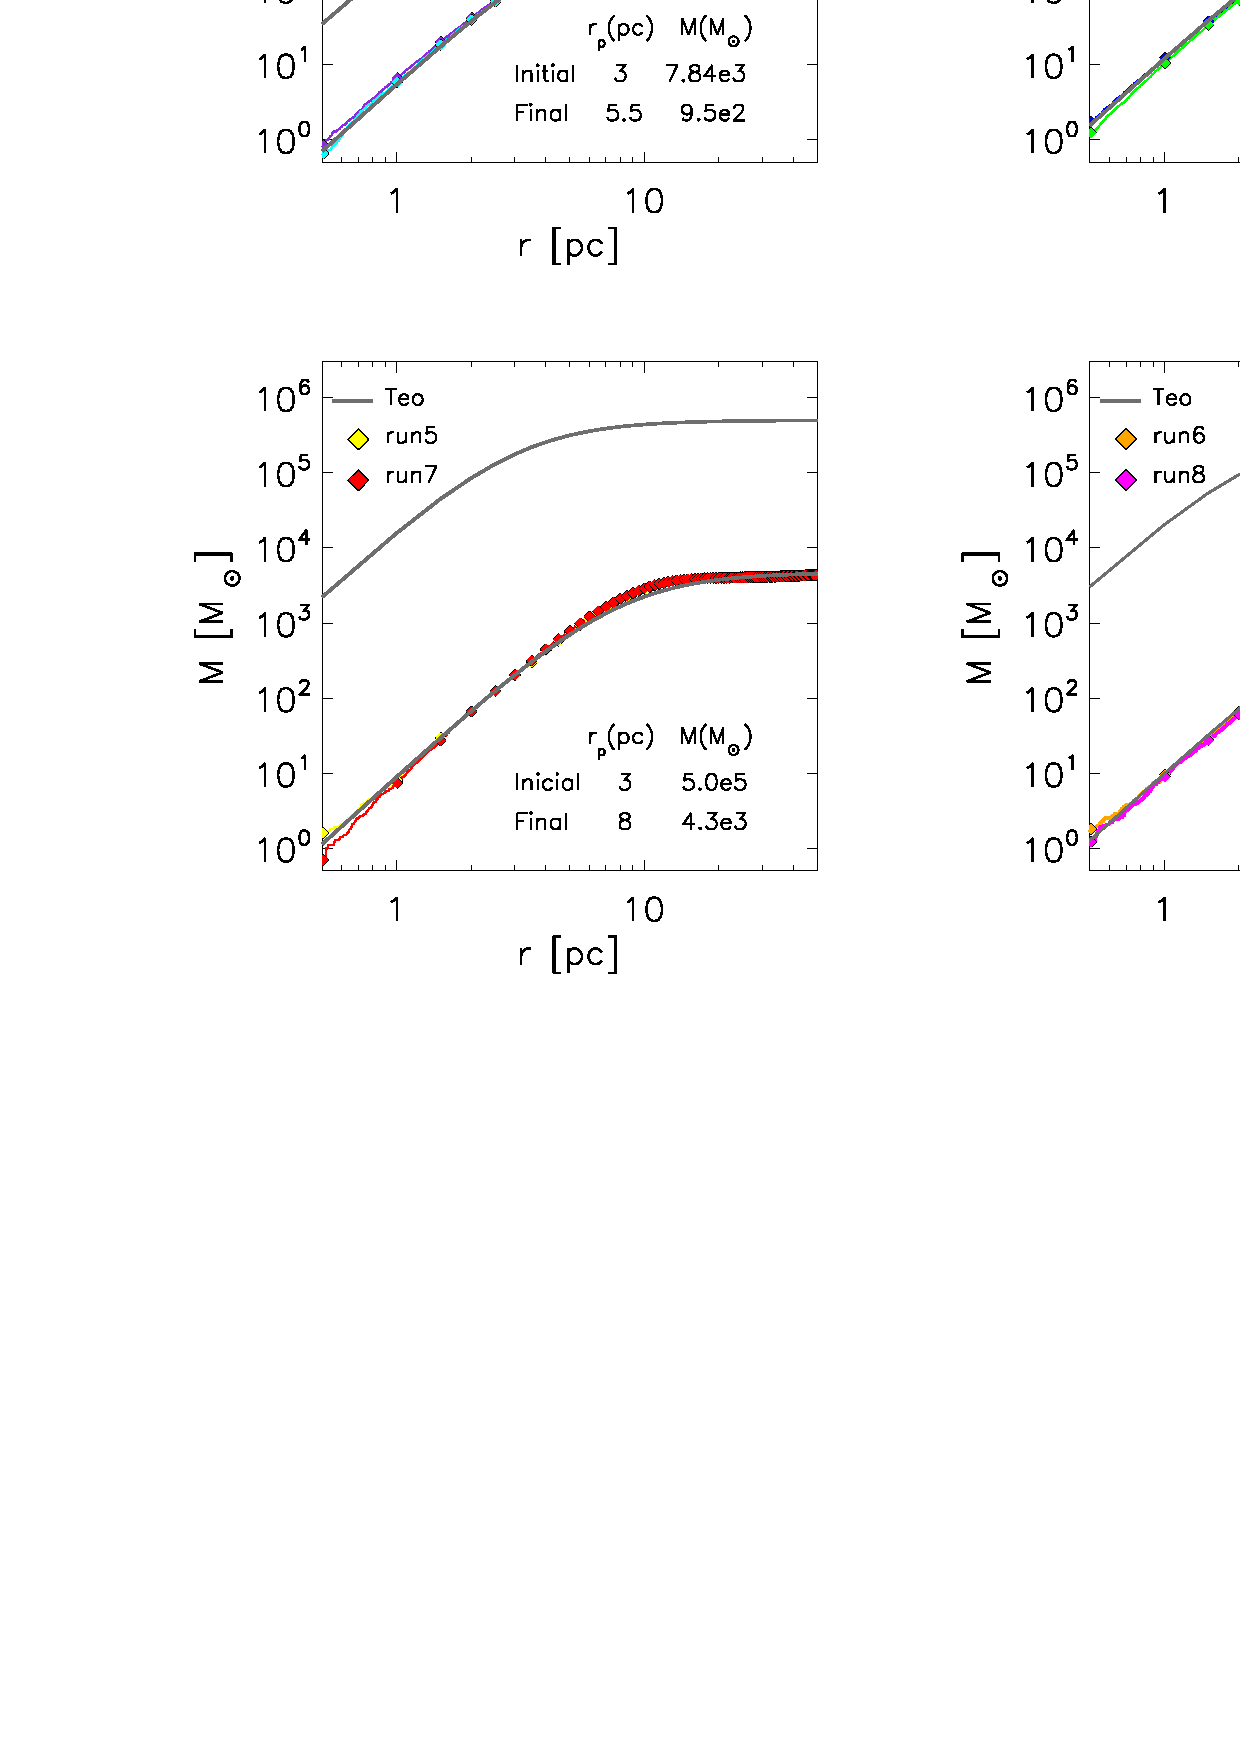
\includegraphics[width=\columnwidth]{Final_Plummer_todo}
  \caption{Example of a simple single-column figure.}
  \label{fig:simple}
\end{figure}




\begin{figure*}[!t]
  \newlength\thisfigwidth
  \setlength\thisfigwidth{0.5\linewidth}
  \addtolength\thisfigwidth{-0.5cm}
  \makebox[\thisfigwidth][l]{\textbf{a}}%
  \hfill%
  \makebox[\thisfigwidth][l]{\textbf{b}}\\[-3ex]
  \parbox[t]{\linewidth}{%
     \vspace{0pt}
     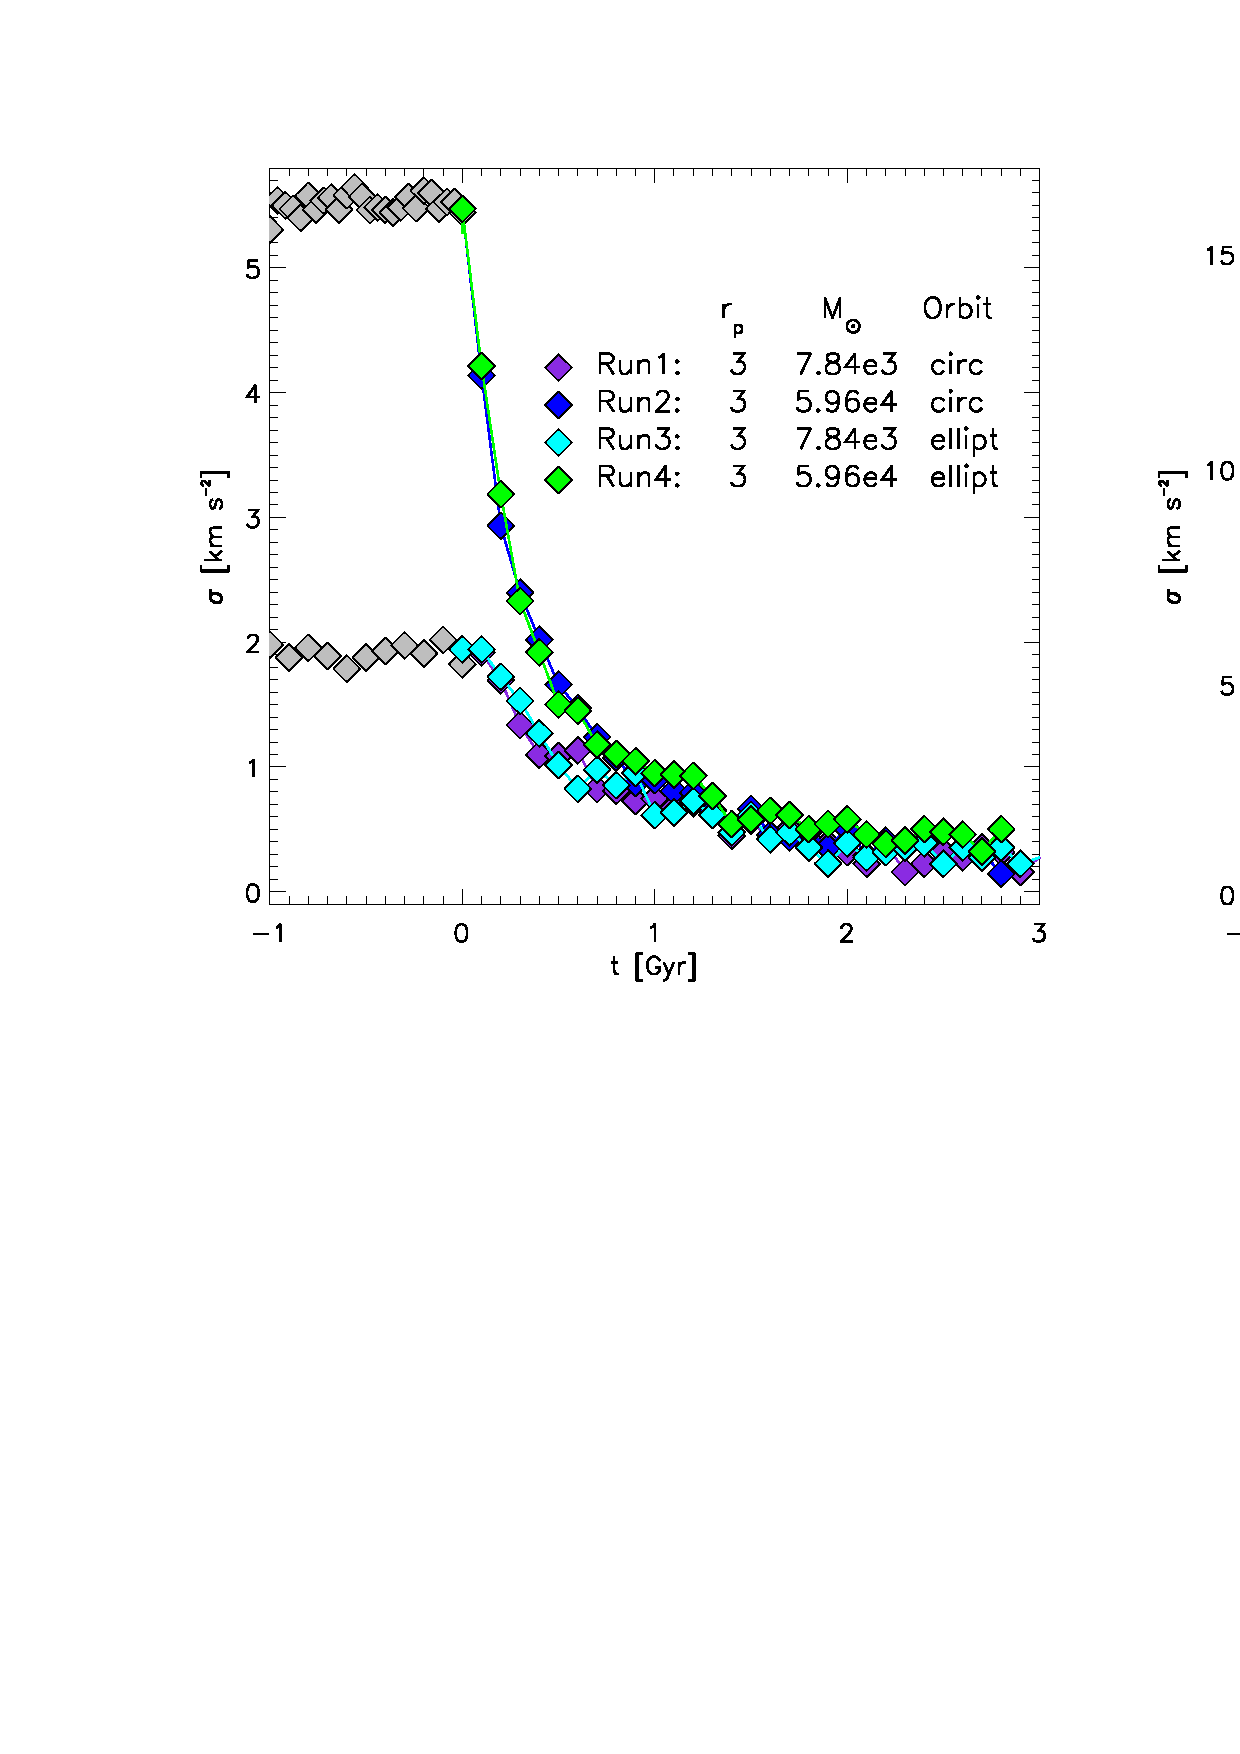
\includegraphics[width=\thisfigwidth,height=3cm]{Disp_todo}%
     \hfill%
     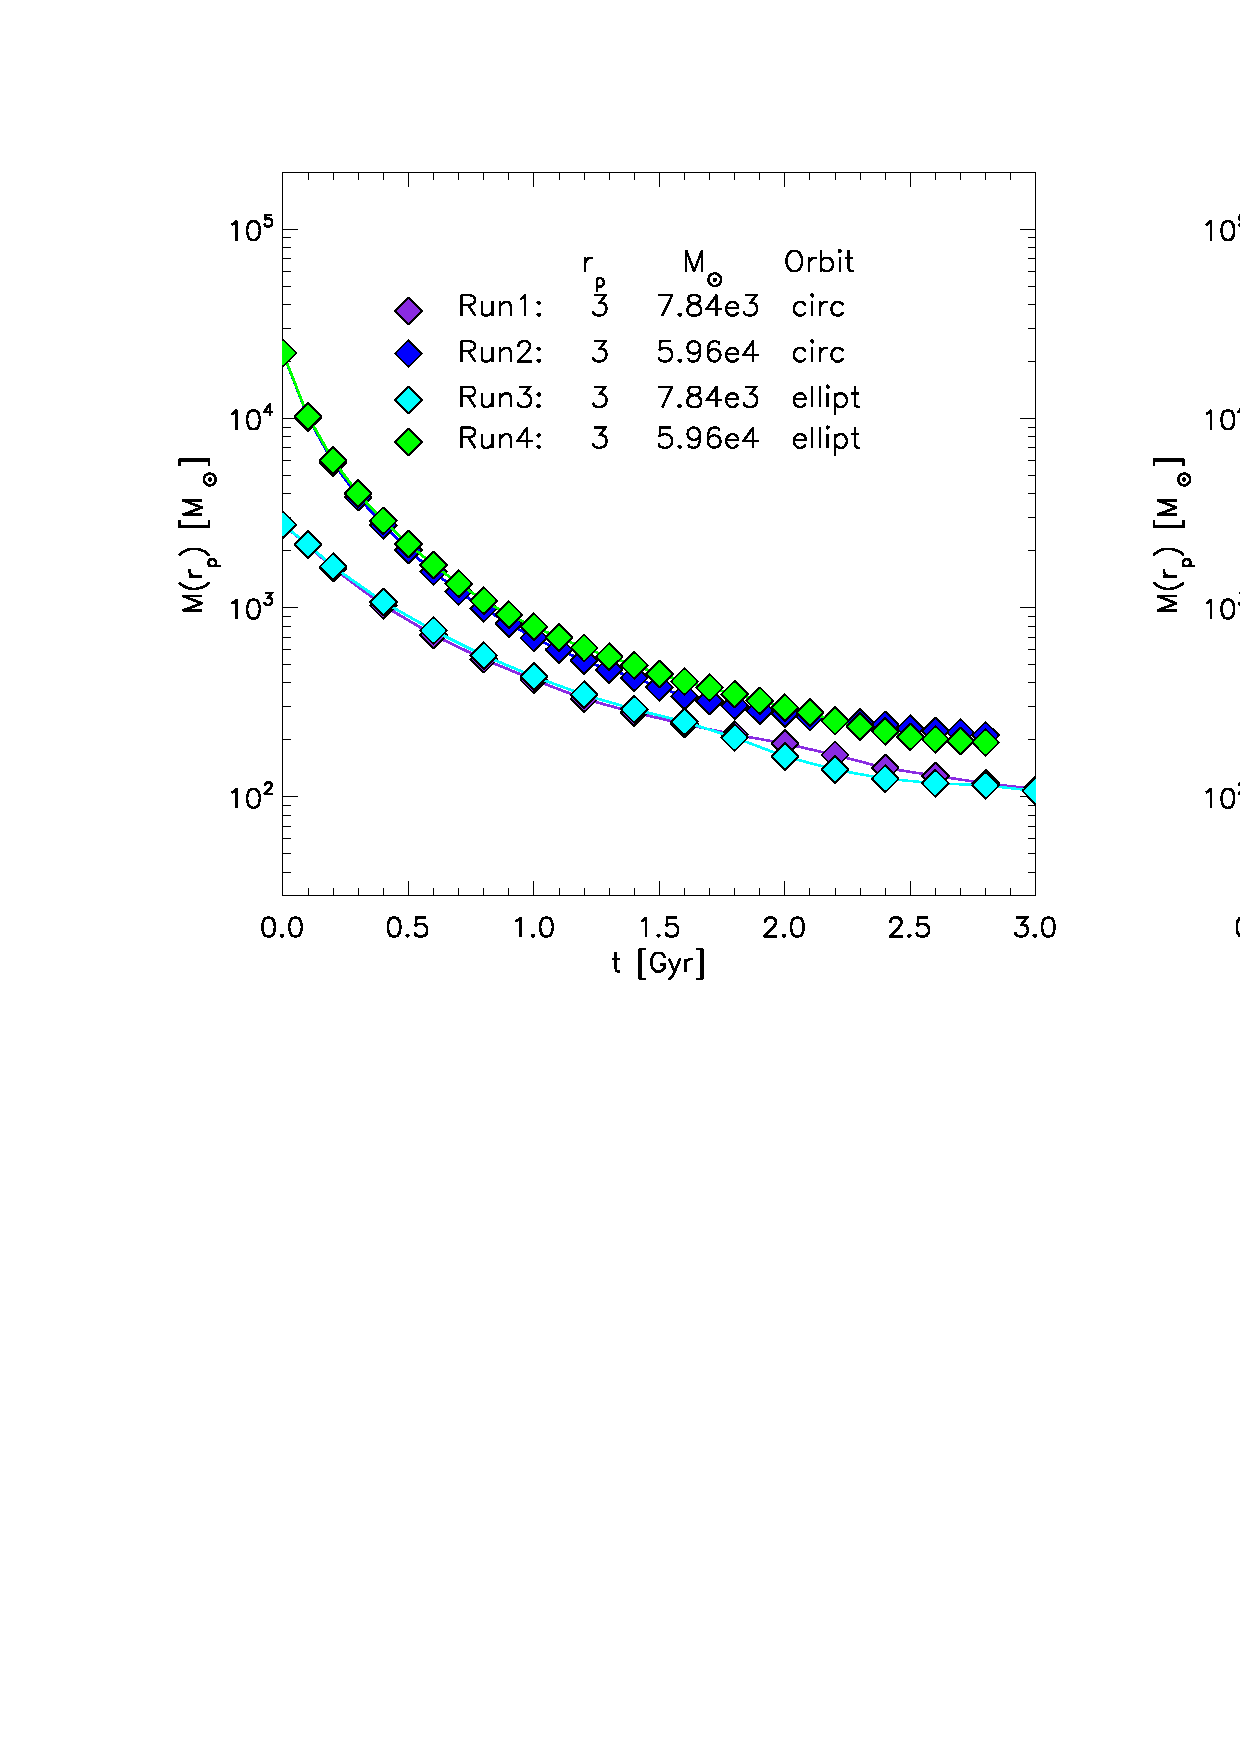
\includegraphics[width=\thisfigwidth,height=3cm]{Mint_todo_lin}
     }
  \caption{A more complicated example of a multipart
    figure, using \LaTeX{} itself to put the \textbf{a} and \textbf{b}
    labels on. (\textit{a}) Multipart figures are captioned like this.
    (\textit{b}) The second part of the figure.  Note that in order to
    align the graphics by their top edges, it is necessary to wrap the
    \CS{includegraphics} commands, preceded by a \CS{vspace\{0pt\}},
    in a \CS{parbox}.  }
  \label{fig:widefig2}
\end{figure*}


%%%%%%%%%
% TABLE %
%%%%%%%%%
\begin{table}[!t]\centering
  \setlength{\tabnotewidth}{0.5\columnwidth}
  \tablecols{3}
  % Stretch the space between table columns 
  \setlength{\tabcolsep}{2.8\tabcolsep}
  \caption{Initial parameters of NGC-6366} \label{tab:ion_ab}
 \begin{tabular}{lrr}
    \toprule
    Model & \multicolumn{1}{c}{$r_{p}$} & \multicolumn{1}{c}{M} \\
          & \multicolumn{1}{c}{[pc]}    & \multicolumn{1}{c}{[$M_{\odot}$]} \\
    \midrule
    run1    & $7.08\pm0.20$ & $6.63\pm0.20$\\
    run2    & $8.08\pm0.14$ & $7.32\pm0.14$\\
    run3    & $8.32\pm0.07$ & $8.02\pm0.07$\\
    run4    & $7.04\pm0.12$ & $6.01\pm0.13$\\
    run5    & $7.59\pm0.11$ & $7.32\pm0.10$\\
    run6    & $6.02\pm0.19$ & $5.47\pm0.20$\\
    run7    & $7.00\pm0.10$ & $6.45\pm0.10$\\
    run8    & $4.93\pm0.16$ & $4.20\pm0.16$\\
    run9    & $6.15\pm0.12$ & $5.55\pm0.14$\\
    run10   &\multicolumn{1}{c}{\nodata} & $5.07\pm0.10$\\
    \bottomrule
    \tabnotetext{a}{Note the use of \CS{lowercase} to prevent the $x$
        from being converted to upper case.}
  \end{tabular}
\end{table}


\section{Conclusions}
\label{sec:conclusions}

\acknowledgments
VL gratefully acknowledges
FJSS gratefully acknowledges

\begin{thebibliography}

\bibitem[\protect\citeauthoryear{Bica et al.}{2016}]{bica:16}
Bica, E., Ortolani, S. \& Barbuy, B.\ 2016, PASA, 33, e028

\bibitem[\protect\citeauthoryear{Campos et al.}{2013}]{campos:13}
Campos, F., Kepler, S.O., Bonatto, C. \& Ducati, J. R.\ 2013, \mnras, 433, 243

\bibitem[\protect\citeauthoryear{Chen \& Chen}{2010}]{chen:10}
Chen, C. W. \& Chen, W. P.\ 2010, \apj, 721, 1790

\bibitem[\protect\citeauthoryear{Helmi et al.}{2018}]{helmi:18}
Gaia Collaboration; Helmi, A. et al.\ 2018, \aap, XXX

\bibitem[\protect\citeauthoryear{Gnedin \& Ostriker}{1997}]{gnedin:97}
Gnedin, O. Y. \& Ostriker, J. P.\ 1997, \apj, 474, 223

\bibitem[\protect\citeauthoryear{Harris}{1996}]{harris:96}
Harris, W. E.\ 1996, \aj, 112, 4

\bibitem[\protect\citeauthoryear{Harris}{2010}]{harris:10}
Harris, W. E.\ 2010, http://physwww.mcmaster.ca/harris/mwgc.dat

\bibitem[\protect\citeauthoryear{McLaughlin \& van der Marel}{2005}]{mclaughlin:05}
McLaughlin, D. E. \& van der Marel, R. P.\ 2005, \apjs, 161, 304

\bibitem[\protect\citeauthoryear{Paust et al.}{2009}]{paust:09}
Paust, N. E. Q. et al., 2009, \aj, 137, 246

\bibitem[\protect\citeauthoryear{Puls et al.}{2018}]{puls:18}
Puls, A. A., Alves-Brito, A., Campos, F., Dias, B. \& Barbuy, B., 2018, \mnras, 476, 690

\end{thebibliography}

\end{document}
